\chapter{Progettazione concettuale}
    \section{Class Diagram del dominio del problema}
    	\begin{figure}[hbt]
  			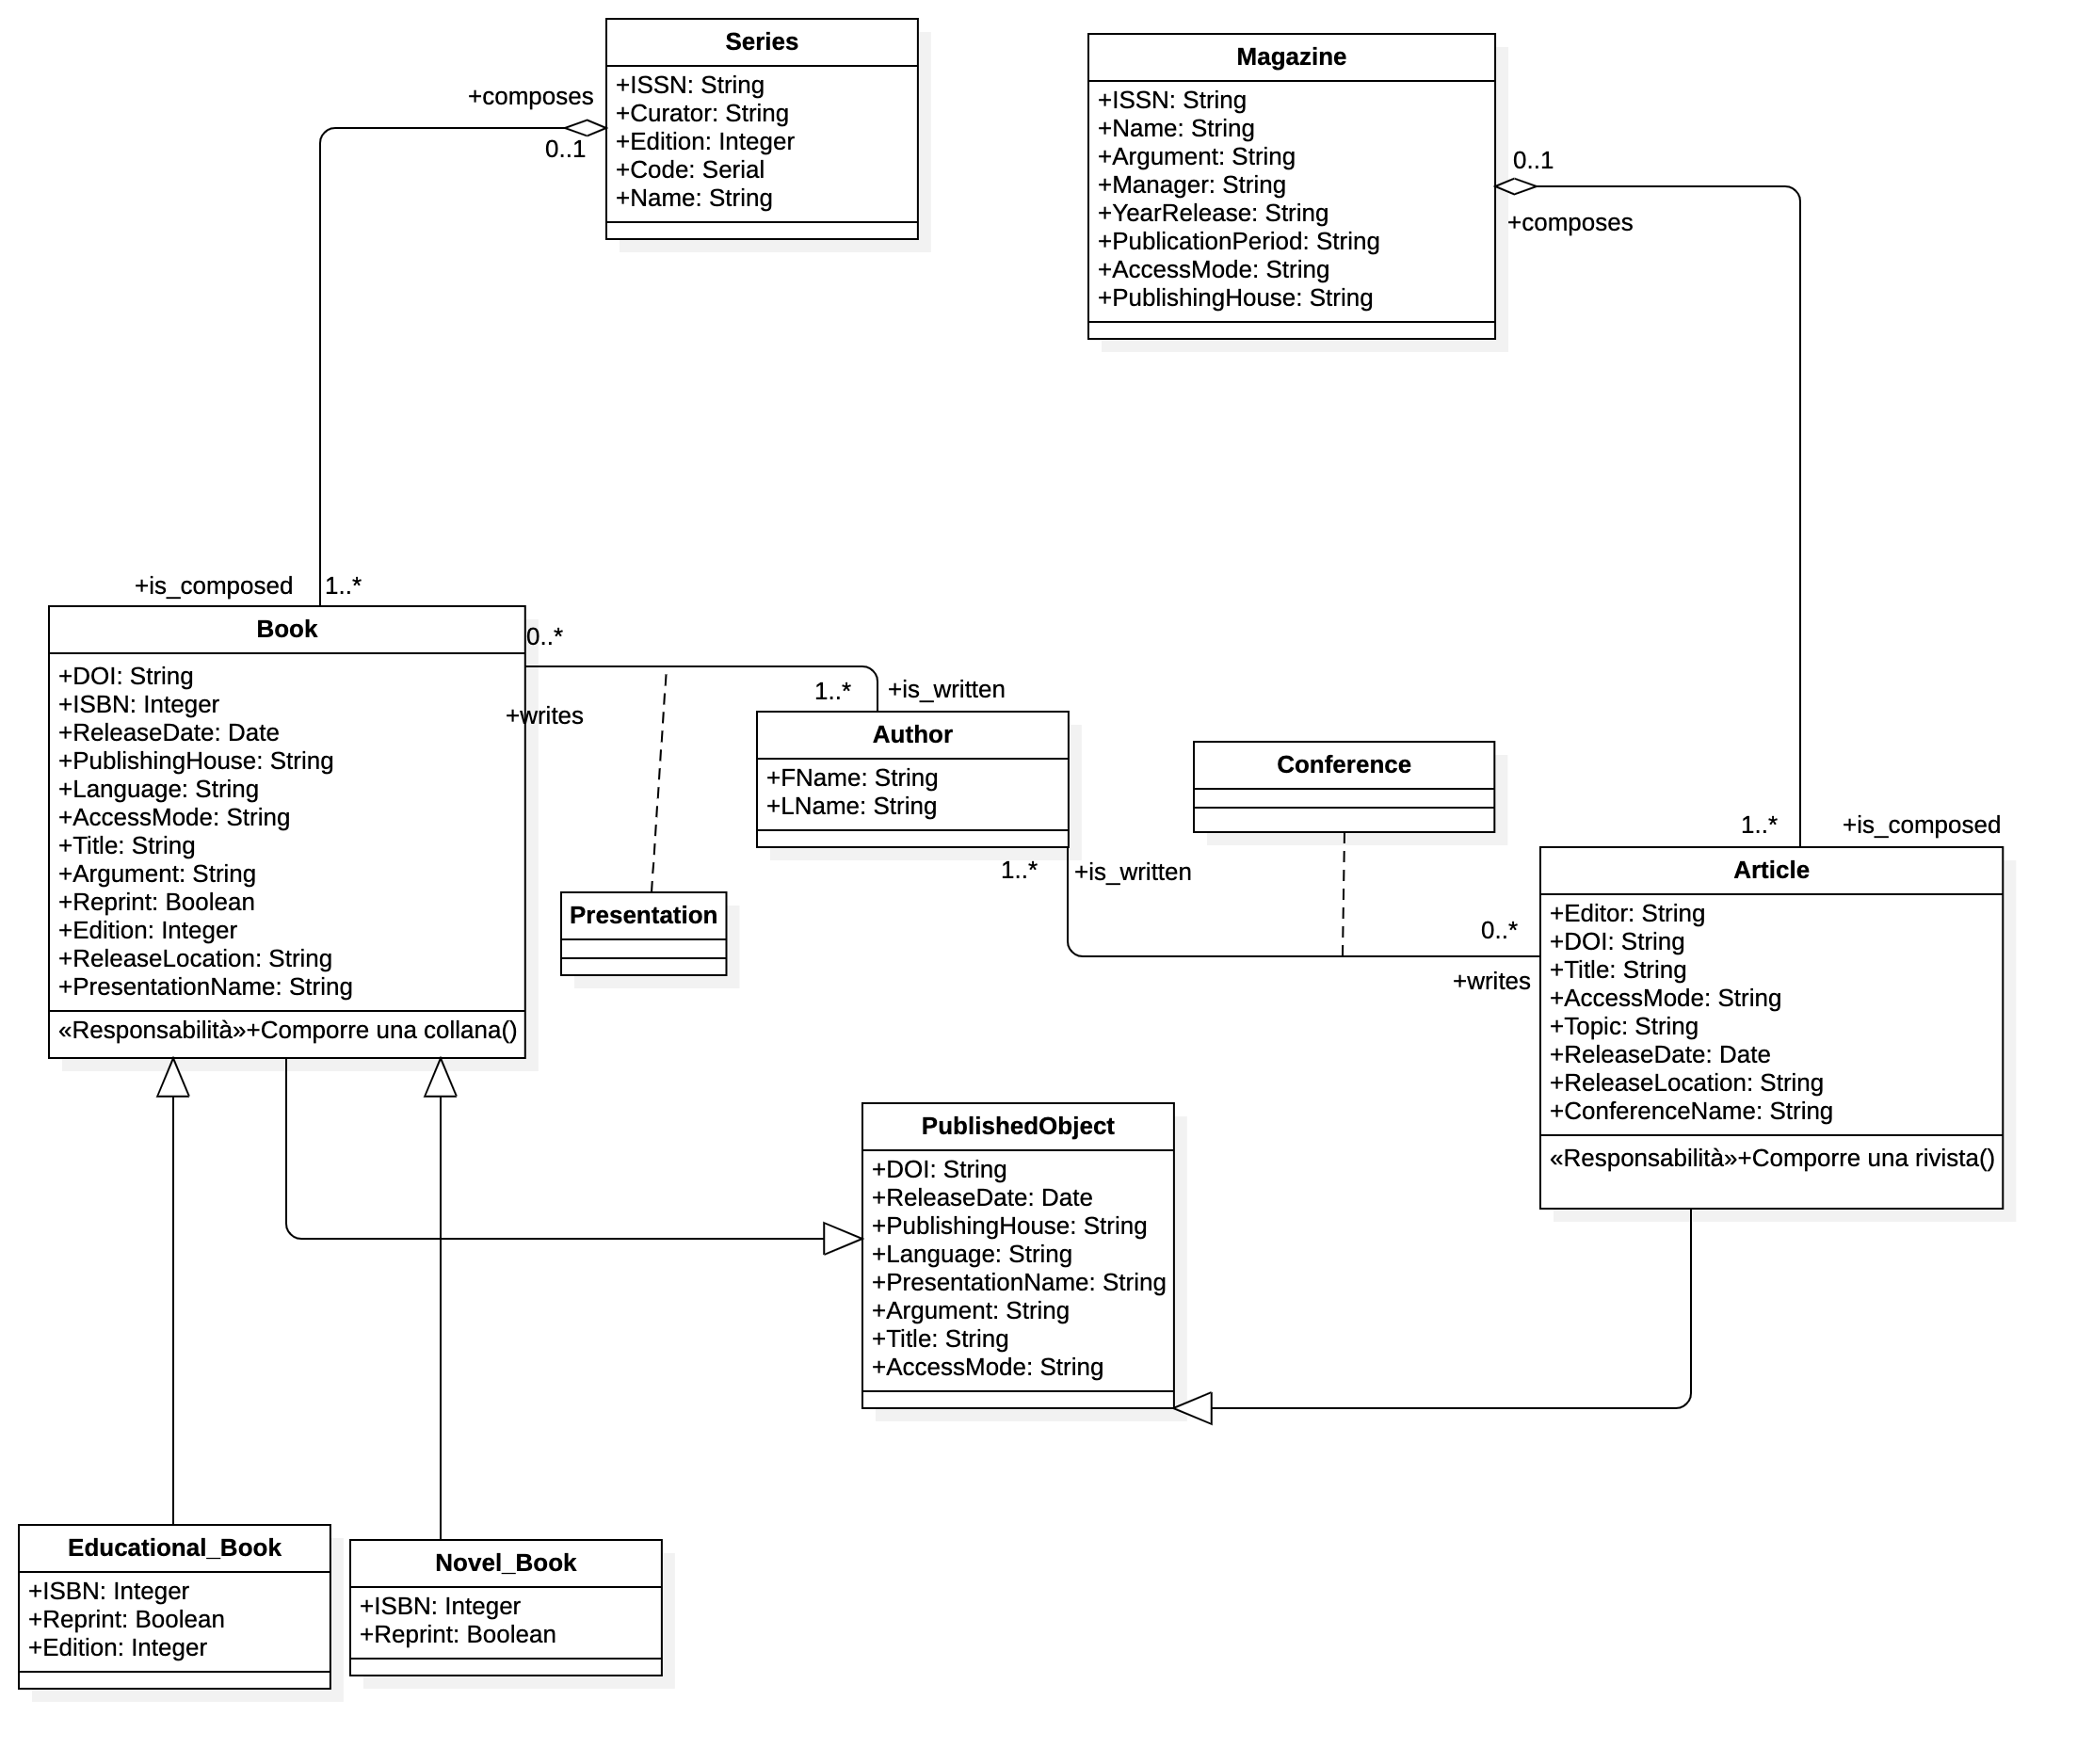
\includegraphics[width=1\textwidth]{/Users/lorenzotecchia/Documents/ESAMI/ProgettoOOBD/ProgettoOOBD_LaTeX_Object/Immagini/CD_DP.png}
  			\caption{Class Diagram del dominio del problema}
	\end{figure}
    \newpage
    \begin{table}[]
\section{Dizionario delle Classi}
\caption{Dizionario delle Classi}

\label{tab:DizionarioClassi}

\resizebox{\textwidth}{!}{%
\begin{tabular}{|l|l|l|}
\hline
\rowcolor[HTML]{E5150C} 
Classe &
  Spiegazione &
  Attributi \\ \hline
\textbf{Author} &
  Autore di libri o articoli &
  \begin{tabular}[c]{@{}l@{}}ID\_Author (Serial): Identificazione dell'autore. \\ FirstName (String): Nome dell'autore. \\ LastName (String): Cognome dell'autore.\end{tabular} \\ \hline
\textbf{Books} &
  \begin{tabular}[c]{@{}l@{}}Oggetti leggibili, romanzi o \\ d'educazione\end{tabular} &
  \begin{tabular}[c]{@{}l@{}}
 	ISBN (Integer): Classificazione numerica di un libto. \\ Edition (Integer): Numero d'edizione. \\ AccessMode (AccessMode): Modo di fruizione. \\ ReleaseDate (Date): Data di pubblicazione. \\ PublishingHouse (String): Casa editrice che ha stampato il libo. \\ ReleaseLocation (String): Luogo di pubblicazione. \\ Language (String): Lingua in cui è scritto il libro.\\ Title (String): Titolo del libor. \\ Argument (String): Argomento del libro. \\ Reprint (Boolean): Parametro che identifica se il libro è una ristampa. \\ PresentationName (String): Nome della presentazione alla quale il libro è presentato.\end{tabular} \\ \hline
\textbf{Series} &
  Insieme di libri &
  \begin{tabular}[c]{@{}l@{}}ISSN (String):Numero internazionale che identifica le collane.\\ Edition (Integer):Numero dell'edizione. \\ Curator (String):Curatore della collana. \\ Code (Serial):Codice affidato alla collana. \\ Name (String): Nome della collana.\end{tabular} \\ \hline
\textbf{Magazine} &
  Insieme di Articoli &
  \begin{tabular}[c]{@{}l@{}}ISSN(Integer):umero internazionale che identifica le riviste. \\ Name (String): Nome della rivista. \\ Argument (String): Argomento della rivista. \\ Manager (String): Manager della rivista. \\ YearRelease (Timestamp): Anno di pubblicazione. \\ PublicationPeriod (String): Periodicità della rivista. \\ AccessMode (AccessMode): Modo di fruizione.\end{tabular} \\ \hline
\textbf{Article} &
  Articoli di ricerca Scientifica &
  \begin{tabular}[c]{@{}l@{}}DOI (String): Digital object Identifier dell'articolo.\\ Title (String): Titolo dell'articolo.\\ AccessMode (AccessMode): Metodo di fruizione.  \\ Editor (String):Editore dell'articolo. \\ ReleaseDate (Timestamp):Data di pubblicazione.\\ ReleaseLocation (String):Luogo di pubblicazione.\\ ConferenceName (String): Nome di conferenza in cui è presentato/discusso l'articolo.\end{tabular} \\ \hline
 \textbf{Conference} & Conferenze in cui vengono discussi gli articoli &
  \begin{tabular}[c]{@{}l@{}} Title(String): Titolo dell'articolo \\ LastName(String): Cognome dell'autore \\ FirstName(String): Nome dell'autore \\ ConferenceName(String): Nome della conferenza \\ReleaseLocation(String): Luogo di rilascio \\ ReleaseDate(Timestamp): Data di rilascio
  \end{tabular} \\ \hline
  
  \textbf{Presentation} & Presentazione in cui vengono presentati i libri &
  \begin{tabular}[c]{@{}l@{}} Title(String): Titolo del libro \\ LastName(String): Cognome dell'autore \\ FirstName(String): Nome dell'autore \\ PresentationName(String): Nome della presentazione \\ReleaseLocation(String): Luogo di rilascio \\ ReleaseDate(Timestamp): Data di rilascio
  \end{tabular} \\ \hline
\end{tabular}%
}
\end{table}


    \begin{table}
\section{Dizionario delle associazioni}
\centering
\caption{Tabella delle Associazioni}
\resizebox{\linewidth}{!}{%
\begin{tabular}{|l|l|l|}    
\hline
\rowcolor[HTML]{E5150C} \multicolumn{1}{|r|}{Nome} & Descrizione                                                                                                                            & Classi Coinvolte  \\
composes/is\_composed                                        & \begin{tabular}[c]{@{}l@{}}Una collana è composta da uno o più libri/\\ Un libro può comporre oppure no una collana\end{tabular}       & Series/Book       \\ 
\hline
writes/is\_written                                           & \begin{tabular}[c]{@{}l@{}}Un libro è scritto da uno o più autori/\\ Un autore scrive molti oppure nessun libro\end{tabular}           & Book/Author       \\ 
\hline
is\_written/writes                                           & \begin{tabular}[c]{@{}l@{}}Un autore scrive molti oppure nessun articolo/\\ Un articolo è scritto da uno o più autori\end{tabular}     & Author/Article    \\ 
\hline
composes/is\_composed                                        & \begin{tabular}[c]{@{}l@{}}Un articolo puo comporre oppure no una rivista/\\ Una rivista è composta da uno o più articoli\end{tabular} & Article/Magazine  \\
\hline
\end{tabular}
}
\end{table}

        
